%%%%%%%%%%%%%%%%%%%%%%%%%%%%%%%%%%%%%%%%%
% University Assignment Title Page 
% LaTeX Template
% Version 1.0 (27/12/12)
%
% This template has been downloaded from:
% http://www.LaTeXTemplates.com
%
% Original author:
% WikiBooks (http://en.wikibooks.org/wiki/LaTeX/Title_Creation)
%
% License:
% CC BY-NC-SA 3.0 (http://creativecommons.org/licenses/by-nc-sa/3.0/)
%
%%%%%%%%%%%%%%%%%%%%%%%%%%%%%%%%%%%%%%%%%
%\title{Title page with logo}
%----------------------------------------------------------------------------------------
%	PACKAGES AND OTHER DOCUMENT CONFIGURATIONS
%----------------------------------------------------------------------------------------

\documentclass[12pt]{article}
\usepackage[english]{babel}
\usepackage[utf8x]{inputenc}
\usepackage{natbib}
\usepackage{amsmath}
\usepackage[colorinlistoftodos]{todonotes}
\usepackage{listings}
\usepackage{color}
\usepackage{tabu}
\tabulinesep=1.2mm
\usepackage[explicit]{titlesec}
\usepackage{url}
\usepackage{subfig}
\usepackage{graphicx}
\usepackage{grffile}
\usepackage{mwe}
\usepackage[section]{placeins}

\definecolor{dkgreen}{rgb}{0,0.6,0}
\definecolor{gray}{rgb}{0.5,0.5,0.5}
\definecolor{mauve}{rgb}{0.58,0,0.82}

\begin{document}

\begin{titlepage}

\newcommand{\HRule}{\rule{\linewidth}{0.5mm}} % Defines a new command for the horizontal lines, change thickness here

\center % Center everything on the page
 
%----------------------------------------------------------------------------------------
%	HEADING SECTIONS
%----------------------------------------------------------------------------------------

\textsc{\LARGE University of St Andrews}\\[1.5cm] % Name of your university/college
\textsc{\Large CS4204 Coursework 1}\\[0.5cm] % Major heading such as course name
\textsc{\large }\\[0.5cm] % Minor heading such as course title

%----------------------------------------------------------------------------------------
%	TITLE SECTION
%----------------------------------------------------------------------------------------

\HRule \\[0.4cm]
{ \huge \bfseries Concurrent Data Structure}\\[0.4cm] % Title of your document
\HRule \\[1.5cm]
 
%----------------------------------------------------------------------------------------
%	AUTHOR SECTION
%----------------------------------------------------------------------------------------


\Large \emph{Author:}\\
 \textsc{150008022}\\[3cm] % Your name

%----------------------------------------------------------------------------------------
%	DATE SECTION
%----------------------------------------------------------------------------------------

{\large \today}\\[2cm] % Date, change the \today to a set date if you want to be precise

%----------------------------------------------------------------------------------------
%	LOGO SECTION
%---------------------------------------------------------------------------------------


\includegraphics[width = 3.1cm]{images/standrewslogo.png}
 
%----------------------------------------------------------------------------------------

\vfill % Fill the rest of the page with whitespace

\end{titlepage}

\part*{Goal}

The goal of this practical was to implement and compare a locking and lock free version of a concurrent account data structure.

\part{Language and Structure}

To allow for thorough analysis, the C language was chosen for this practical. This would allow both data structure implementations to use fairly low level operations whilst maintaining a reasonable level of readability and ease of development. Since the gcc compiler can also provide the resulting assembly code, this could also be analysed when comparing lock free and locking implementations. Comparing the effects of compiler optimisation on the locking code could also be considered. 

The interface for the account is provided in \emph{account.h}. Since C doesn't support classes, the methods described in the practical specification were altered to also take an account pointer as an argument. Create and destroy methods were also provided to allocate and free any memory used by the account struct.

\part{Locking}

The locking account struct involved two fields, the account balance and the account lock. This lock would have to be obtained in order for a method to make changes to the balance. The account creation method would initialise the mutex with the default attributes. The default provides blocking behaviour, where the thread will wait until it's able to obtain the lock. The mutex initialisation is included in the creation method to avoid multiple threads trying to initialise the lock later when it becomes needed.

Each method for interacting with the account struct first obtains the lock. This is necessary to ensure that the balance variable will not be written to while reading, or written to by multiple threads simultaneously. The implementation is analagous to using the Synchronised keyword on each method in Java as essentially only one thread can operate on the object at any one time. Initially, a lock was not required for reading as it was assumed that the read would be atomic in the sense that a write could not happen simulatenously and return the half-written value at the relevant memory address. However, further reading showed that this behaviour was undefined, since this kind of atomic read for word-sized variables (i.e. int) was completely dependent on the compiler and architecture of the system \cite{mutexAtomic}. 

For the destruction method, it is assumed that this would be called once all threads are finished operating on it. Realistically, there should be checks for success after calling the \emph{pthread\_mutex\_destroy} method as destroying a mutex that is currently held by another thread can produce undefined behaviour \cite{mutexUndefined}.

The locking mechanism has the potential to suffer from the stampede issue discussed in lecture, and so another implementation was provided that used exponential backoff to try and mitigate this issue. This was done by adding a function for obtaining the lock, which would initially wait a given time before trying again, and double this delay after each failure. A maximum was set to avoid ridiculous wait times which when reached reset the delay back to the initial value. To avoid stampedes still occuring when wait times synchronised between threads, a random multiplier could also be used, but was not included in this implementation.

Since the lock is obtained and released within each method, it is not possible for a thread to hold multiple locks, or wait on another lock while holding one. Because of this, deadlock is not possible. 

The lock implementation can be compiled by running \emph{make locking} to produce the executable, and the backoff implementation by running \emph{make locking\_backoff}. 

\part{Lock Free}

The lock free account structure remained the same, but without the mutex. Since mutexes are surprisingly large on linux systems (24 bytes on 32-bit machines, and 40 bytes on 64-bit machines \cite{mutexSize}), this already had advantages in terms of memory requirements. 

The \emph{atomic\_compare\_exchange\_weak} builtin from \emph{stdatomic.h} was used to provide lock free concurrent access to the balance. A simple while loop would check if the value in expected matches the desired value, and try again if not. Since the atomic function would write the actual value to the expected variable if the values did not match, the loop could try continuously.

Possible issues with this implementation is the potential waste of resources caused by the constant spinning. Another possible issue is the ABA problem. This would occur if the following events occurred: 

\begin{enumerate}
\item Process 1 reads the current value of a variable to be A.
\item Process 2 takes over execution, and writes B to the variable, and then A
\item Process 1 returns to execution, and reads A, and assumes nothing has changed inbetween.
\end{enumerate}

This would not be a problem for the simple account data structure, since the history of the account would not matter. However, this problem would have to be taken into account when designing systems that rely on nothing changing between the two reads by process 1.

The lock free implementation can be compiled by running \emph{make lockfree}.

\pagebreak
\part{Tests}

All experiments were run on a machine with the specification shown in table \ref{sysarchitecture}.
\begin{table}

\begin{center}
\begin{tabu} to 1.0 \textwidth { | X[l] | X[l] | }
 \hline
 Model Name  & Intel(R) Core(TM) i7-8750H CPU \\ 
 \hline
 Clock Speed & 2.20GHz \\
 \hline
 Architecture  & x86\_64 \\
 \hline
 CPU(s)    & 12 \\
 \hline
 Thread(s) per Core & 2 \\
 \hline
 Socket(s) & 1 \\
 \hline 
 Core(s) per socket & 6 \\
 \hline
 OS       & Ubuntu 18.04 \\
 \hline
\end{tabu}
\caption{Test System Architecture}
\label{sysarchitecture}
\end{center}
\end{table}

\section{Correctness}

To test the correctness of the different implementations, each of them were run with an increasing number of threads. Each thread knew its index in the pthread\_t array, and so even indices would withdraw from the account and odd would deposit. All threads would repeat this action 1000 times before terminating printing what they "see" as the current value of the variable to ensure that the operation was occuring correctly.

Both implementations showed no errors, and the end values were as expected. 

Out of curiosity, the same method was written to use the deprecated \url{__sync_bool_compare_and_swap} builtin, which is the version used in the submission. The compiler is meant to fall back to \_\_sync\_ when 'neccessary'. Comparing the assembly code generated by both implementations, it was observed that both used the \url{lock cmpxchgl} instructions. The \url{cmpxchgl} instruction is responsible for the compare and swap. The documentation mentions that for multiple processor systems, the \url{lock} prefix must be used to ensure that the compare and exchange is atomic \cite{intelAtomic}. To ensure compatability with other architectures however, the atomics method would be preferred.

More thorough testing of correctness would involve performing the same tests on multiple varied architectures. Exhaustive modelling methods such as PROMELA would also provide assurance the compare and swap mechansism was correct.

\section{Performance}

To test performance, two aspects were considered:

\begin{itemize}
\item Wait time: how long does a requesting thread spend waiting to carry out an operation.
\item Number of retries: how many iterations of attempting to access the resource before success.
\end{itemize}

\noindent These metrics were compared as the number of competeting threads were increased.

Increasing the number of threads far past the number of threads that can be processed simultaneously would increase the effect of the scheduler on the results. Therefore equation \ref{eq:nthreads} was used to calculate the maximum number of simulateonously processable threads. For the architecture described earlier, $\textit{nthreads}_\textit{max} = 12 $. Up to 24 threads were used in the experiment out of curiosity, though the calculated value would be considered during analysis.

\begin{equation}
\label{eq:nthreads}
	\textit{nthreads}_\textit{max} =
	 \textit{threads per core} \times \textit{cores per socket} \times \textit{number of sockets}
\end{equation}

Since the backoff lock could only use nanoseconds as the smallest unit, it was not possible to use values for maximum and initial delay that would be able to compete with the other lock implementations.

\subsection{Setup}

In order to capture the data needed, the functions would have to be slightly changed to capture the behaviour needed, and the process of recording data would have to be as unintrusive as possible. 

This was achieved by passing an \url{Attempt} struct to each of the \url{CAccount} methods so that the number of attempts could be recorded. This would only add a few extra clock cycles after each attempt to gain the lock.

The CPU clock time before and after the function call was used to obtain the time taken for the function to execute, and provide a rough value for the wait time.

Before each experiement, memory was allocated for all the \url{Attempt} structs required for each thread, and freed afterwards. The max, min, and average values would be obtained for each thread, and printed to the console. To store the results, stdin was redirected to a csv file.

\subsection{Analysis}

To analyse and create plots of the data, a python script was used. The independant variable in each graph would be the number of threads, and this was plotted against the average, max, and minimum number of retries and wait times.

The data generated was manually checked for error before being transformed and grouped by experiment for easier manipulation in python.

A scatter plot was created of each dependant variable against the independant variable. Plots merging the results from the different locking mechanisms were also created. In order to improve the visualisations, the wait times were converted from seconds to nano seconds, as the former appeared as a flat line when plotted due to the automatic scaling provided by matplotlib. 

Once plotted, it was realised that the minimum wait time and number of tries was constant for all threads, and so this was omitted from the results.

\subsection{Results}

In each plot, each point corresponds to the measurement made by an individual thread when using a specific locking mechanism, i.e. when using two threads, there will be two data points for each locking mechanism at $x = 2$.

Figure \ref{fig:mergedavgwait} shows that there is a large performance difference between each mechanism. The backoff implementation had the largest variance as the number of threads increased, and the lockfree implementation had the best performance overall. Locking showed a linear growth in wait time, whilst lockfree showed logarithmic growth.

\begin{figure}[!h]
\centering
  \centering
	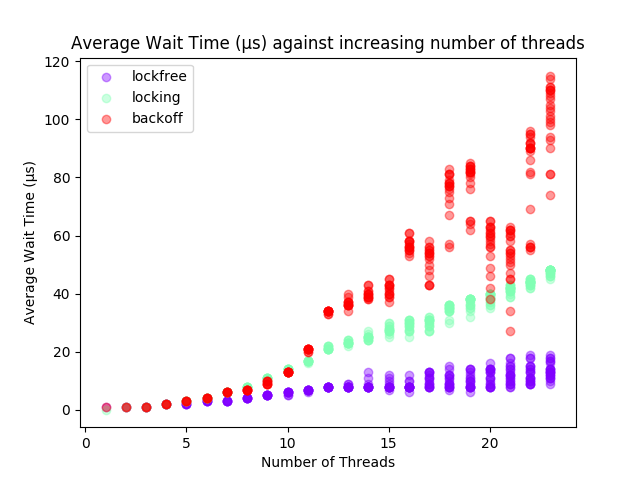
\includegraphics[width=0.8\linewidth]{images/mergedAverageWait}
	\caption{Average wait time of all locking mechanisms}
	\label{fig:mergedavgwait}
\end{figure}

Since the larger unit of delay used in the backoff implementation affected the scale of the plot in Figure \ref{fig:mergedavgwait}, Figure \ref{fig:omittedavgwait} was also made. By only considering up to $x = 12$, we can see that the lockfree mechanism produces the lowest wait time once more than 4 threads are involved. The effect of the scheduler can also be seen once $x > 12$, as the variance of the average wait times for both locking mechanisms increases. 

\begin{figure}[!h]
  \centering
  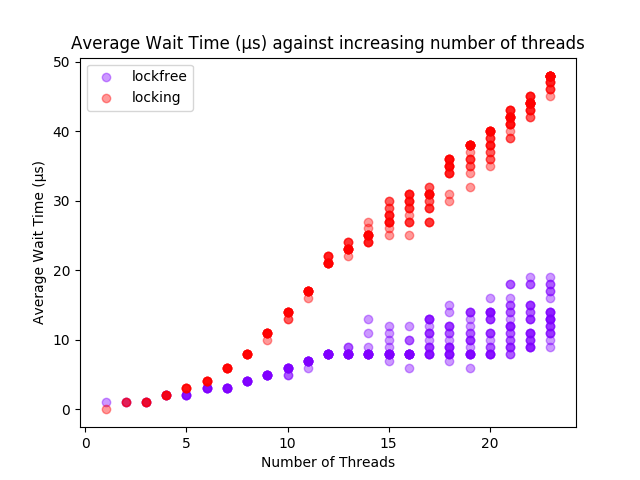
\includegraphics[width=0.8\linewidth]{images/omittedAverageWait}
	\caption{Average wait time of locking and lockfree locking mechanisms}
  \label{fig:omittedavgwait}
\end{figure}

Whilst the lockfree mechanism appears to reduce the time spent waiting to access a resource, the mutex has the advantage of allowing a thread to sleep, and allowing other threads to continue execution whilst it does so. Since the lockfree implenentation requires constant polling of the resource, it is likely to be less energy effecient, and more demanding on the CPU. Though the backoff implementation was expected to reduce these negatives, it would suffer the trade-off of likely increasing average wait times.

Figure \ref{fig:mergeavgtries} proves this tradeoff up until $x = 12$, at which point the backoff implemenetation begins performing far worse. Since the locking implementation would only ever try to obtain the lock 'once' before sleeping and then wait until the scheduler woke the thread once the lock was available, it would appear to only ever make on attempt. 

\begin{figure}[!h]
  \centering
  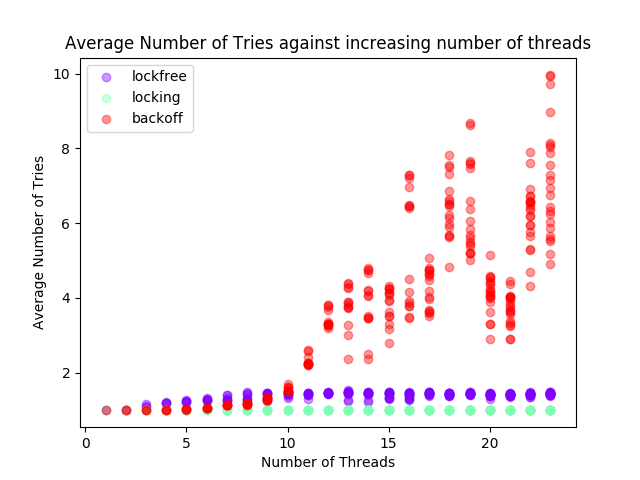
\includegraphics[width=0.8\linewidth]{images/mergedavgtries}
	\caption{Average number of tries of all locking mechanisms}
  \label{fig:mergeavgtries}
  
\end{figure}
Interestingly, the average number of attempts to update the resource was also fairly constant with the lockfree implementation. In Figure \ref{fig:omittedavgtries}, it is clear that the average number of tries for the lockfree data structure sits only just above the mutex approach. Figure \ref{fig:omittedmaxtries} shows that the maximum number of tries grows linearly with the number of threads for the lock free approach, but since the average remains at around 1.5 tries, these worst cases must appear infrequently. 

In figure \ref{fig:omittedmaxtries}, it was also noticed that the maximum number of tries did not grow once $x > 12$. This was explained by considering the fact that it would only be possible for 12 threads in this architecture to be writing to the data structure at once. Since linux uses the "Completely Fair Scheduler" (CFC) \cite{cfc}, the thread with the least execution time will be chosen next to run. Therefore, after the first 12 threads have run in parallel and carried out the withdraw or deposit functions, it is likely that the other waiting threads would be executed next and would only be competeting with each other, rather than the full set of threads currently in execution.

\begin{figure}[!ht]
  \centering
  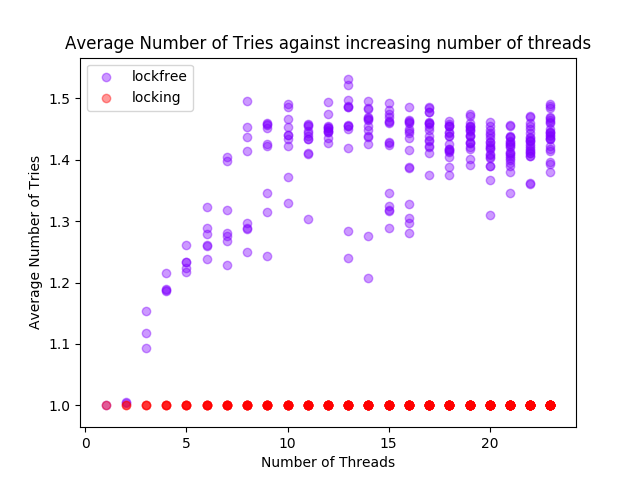
\includegraphics[width=0.8\linewidth]{images/omittedavgtries}
	\caption{Average number of tries for locking and lockfree mechanisms}
  \label{fig:omittedavgtries}
\end{figure}

\begin{figure}[!ht]
  \centering
  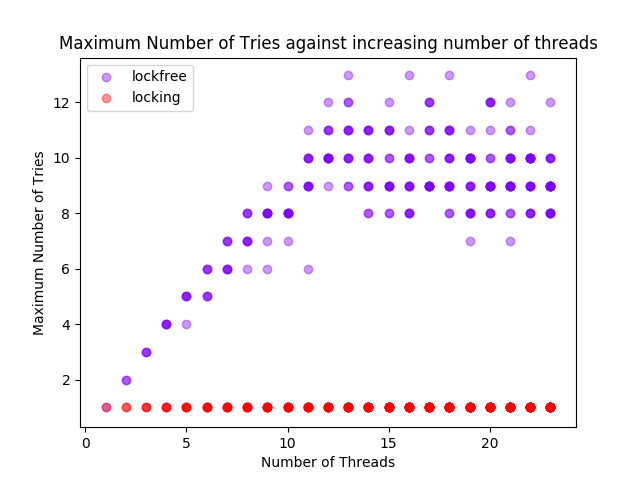
\includegraphics[width=0.8\linewidth]{images/omittedmaxtries}
	\caption{Maximum number of tries of locking and lockfree mechanisms}
  \label{fig:omittedmaxtries}
\end{figure}

\part*{Conclusion}

The practical proved an interesting insight into alternatives to mutexes and their pros and cons. Analysis of the results strengthened my understanding of multithreading and scheduling. It also provided an opportunity to refresh my understanding of C, and build my confidence in developing multithreaded C programs.

Given more time, I would have liked to carry out the experiments on multiple architectures as discussed earlier for comparison. For example, it would be intersting to see if on a machine with far more or far fewer cores, would compare and swap still prove more effective. 

I would also like to have compared different types of mutexes, as only two implementations were tested in this practical (timeout and exclusive). 

\bibliographystyle{unsrt}
\bibliography{mybib}

\end{document}
